\documentclass[11pt,a4paper]{article}

\usepackage[utf8]{inputenc} 
\usepackage[T1]{fontenc} 
\usepackage{lmodern}
\usepackage[margin=2cm]{geometry}
\usepackage[german]{babel}
\usepackage{array}
\setlength{\parindent}{0pt}
\setlength{\parskip}{1ex plus 0.5ex minus 0.5ex}

\usepackage{amsmath} 
\usepackage{graphicx} 
\usepackage{booktabs}
\usepackage[colorlinks]{hyperref}
\usepackage{nicefrac}
\usepackage{gensymb}
\usepackage[usenames,dvipsnames,svgnames,table]{xcolor}

\hbadness=99999

\begin{document}

{
\centering 
\large 
Physiklabor für Anf\"anger*innen \\
Ferienpraktikum im Sommersemester 2018 \\[4mm]
\textbf{\LARGE 
Versuch 38: Wärmekapazität
} \\[3mm]
(durchgef\"uhrt am 10.09.2018 bei Nico Strauß) \\
Andréz Gockel, Patrick M\"unnich\\
\today \\[10mm]
}

\section{Ziel des Versuchs}

Der Versuch ist in zwei Teile geteilt, welche dazu dienen, die Wärmekapazität von Wasser zu bestimmen. Im Teil A bestimmt man die Temperatur Differenz von Wasser während der Umwandlung von mechanischer Energie zu thermischer Energie durch Reibkräfte mit Hilfe des Schürholz-Apparates. Im Teil B verwendet man einen elektrischen Widerstand um elektrische Leistung über ein bestimmten Zeitraum in thermische Energie zu wandeln.

\section{Auswertung und Fehleranalyse}

\subsection{Teil A - Umwandlung von mechanischer Arbeit in Wärme }
$$
\begin{array}{lc}
	\multicolumn{1}{l}{\textrm{Zu Bestimmende Werte}} \\
	\hline
	\textrm{Masse Wasser} & m_W \\
	\textrm{Masse Kalorimeter} & m_{kal} \\
	\textrm{Umdrehung} & n \\
	\textrm{Temperatur} & \Delta T\\
	\textrm{Durchmesser Kalorimeter} & d\\
\end{array}
\qquad
\begin{array}{p{3.5cm}l c}
	\multicolumn{2}{l}{\textrm{Bekannte Werte (Fehler nicht-beitragend)}} \\
	\hline
	\textrm{Spezifische Wärme\-kapazität Kupfer} & c_{Cu} = 0.38\, \nicefrac{\textrm{kJ}}{\textrm{(kgK)}} \\
	\textrm{Wärmekapazität vom Nylonseil} & C_T = 5\, \nicefrac{\textrm{J}}{\textrm{K}} \\
	\textrm{Masse Gewicht} & m = 5\, \textrm{kg} \\
\end{array}
$$

\subsubsection{Aufgabenstellung}

\begin{figure}[h]
\begin{minipage}{.6\textwidth}
	Mit Hilfe von dem Sch\"urholz Apparat ist die W\"armekapazit\"at von Wasser zu bestimmen. Dies wird getan, indem man ein Nylonseil \"uber ein mit $50$ ml Wasser gef\"ullten Kaloritmeter windet, ein Thermometer dranschraubt und am Ende des Nylonseils eine $5$ kg Masse dranh\"angt. Das Kalorimeter wird gedreht, sodass die Feder vom Sch\"urholz Apparat entspannt ist, also die Reibkraft $F_R$ die Gewichtskraft $F_G$ ausgleicht. Die Temperatur wird beim Drehen gemessen und notiert.
\end{minipage}%
\begin{minipage}{.4\textwidth}
\centering
\fbox{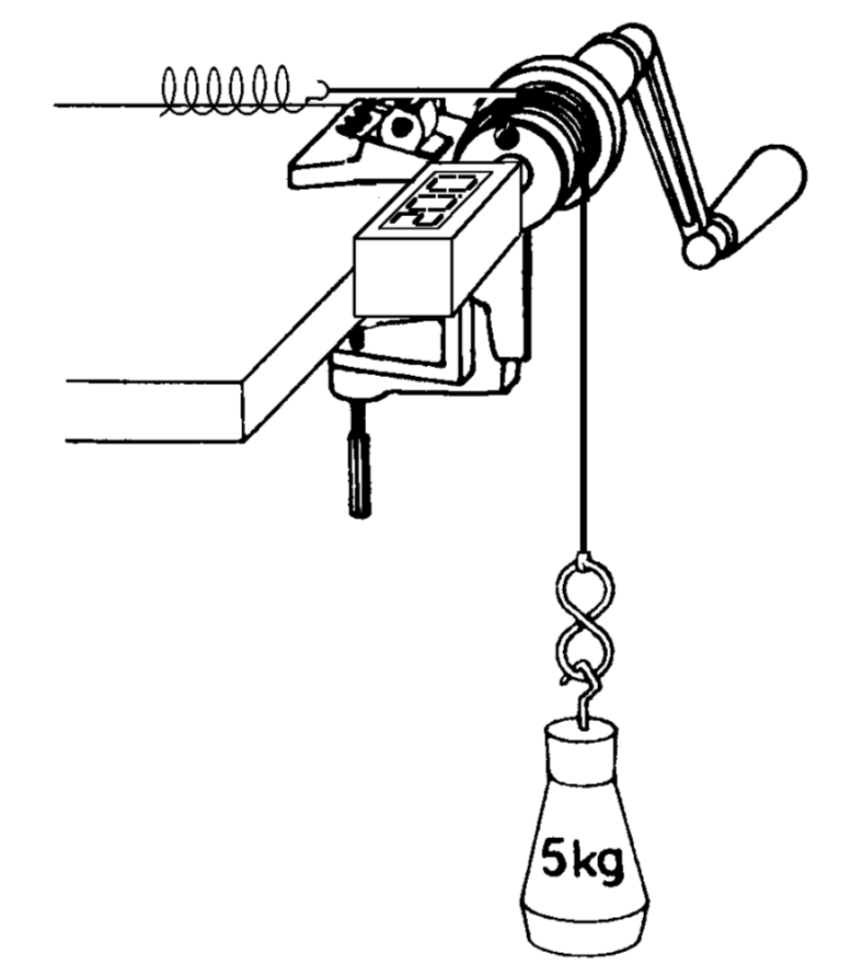
\includegraphics[width=0.5\textwidth]{SchurSketch}}
   \renewcommand\thefigure{B1}
\caption{Schürholz Apparat}
\label{JS1}
\end{minipage}
\end{figure}

\subsubsection{Auswertung}

Die Messung wurde zweimal durchgef\"uhrt. Bei der ersten Durchf\"uhrung wurde die Temperatur\"anderung \"uber 50 Drehungen jeweils im Abstand von 10 Drehungen gemessen. Die zweite Durchf\"uhrung wurde mit 100 Drehungen durchgef\"uhrt und die Temperatur alle 5 Drehungen notiert. Die genauen Messwerte befinden sich im Anhang. \ref{table:m1}, \ref{table:m2}.

Die restlichen Messungen ergaben: $$m_W = 79.18(3)\,\textrm{g}, \quad m_{kal} = 98.05(3)\,\textrm{g}, \quad d = 4.765(3)\,\textrm{cm}$$

F\"ur die W\"armekapazit\"at gilt:\\

\begin{equation}
C=C_{Kal}+C_T+m_wc_w,\label{eq1}
\end{equation}

was umgestellt werden kann zu:

\begin{equation}
c_w=\frac{C-C_{Kal}-C_T}{m_w}.\label{eq2}
\end{equation}

$C$ wird hier mittels der folgenden Gleichungen bestimmt:

\begin{equation}
C=\frac{Q}{\Delta T}
\end{equation}

\begin{equation}
W_R=mgn\pi d=Q
\end{equation}

Mit unseren Messwerten und dem $uncertainties$ Paket in Python berechnen wir damit:\\
$$\begin{tabular}{|c|c|c|c|c|}
\hline
\textrm{Messung} & 1 & 2 & \textrm{Mittelwert} & \textrm{Gewichtet} \\ 
\hline
\textrm{W\"armekapazit\"at} $\left[\mathrm{\nicefrac{\mathrm{J}}{kg K}}\right]$ & $8300\pm1400$ & $3500\pm600$ & $5900\pm800$ & $4187\pm 554$ \\
\hline
\end{tabular}$$

Diese Rechnungen wurden mit dem \textit{uncertainties} Paket in Python durchgef\"uhrt. Diese Rechnungen k\"onnen im Anhang gefunden werden..\\

Der Fehler der Messung mit dem Sch\"urholz Apparat ist aufgrund der gro\ss en Ungenauigkeit der Temperatur und der Anzahl Drehungen sehr gro\ss. Au\ss erdem ist es recht wahrscheinlich, dass $F_{R}$ und $F_{G}$ sich nicht st\"andig ganz ausgleichen, also dadurch auch eine Unsicherheit entsteht. Dies ist einflussreich, da die W\"arme, $Q$, von $F_R$ via $W_R=\int F_Rds$ abh\"angig ist. Da $F_R$ \"uber $F_G$ bestimmt wird und dies bei nicht korrekter Ausgleichung der Beiden nicht akkurat ist, ist also auch $Q$ und dadurch $c_w$ ungenau. Als systematischer Fehler kommt noch die Ungenauigkeit der Masse von 5\,kg hinzu. Der Literaturwert hierzu ist $4182$ $\mathrm{\nicefrac{\mathrm{J}}{kg K}}$. Der Unterschied beim normalen Mittelwert ist aufgrund der Messungenauigkeiten und niedrigen Anzahl Messungen sehr gro\ss.\\

Der gewichtete arithmetische Mittelwert ist jedoch sehr nahe an dem Literaturwert. Dies der Fall, da die zweite Messung wesentlich n\"aher dran ist und der Fehler dort wesentlich kleiner ist. Aufgrund der Formel f\"ur den gewichteten arithmetischn Mittelwert,

\begin{equation}
\overline{x}_g=\frac{\sum_ig_ix_i}{\sum_ig_i},
\end{equation}

mit den Gewichtsfaktoren

\begin{equation}
g_i=u_i^{-2},
\end{equation}

wird hier also der zweite Wert st\"arker gewichtet und wir bekommen einen Mittelwert, der um $0.009\,\sigma$ vom Literaturwert abweicht. Dies wurde mit 

\begin{equation}
t=\frac{|x_0-y|}{u_x}\label{abw}
\end{equation}

berechnet.

\pagebreak

\subsection{Teil B - Umwandlung von elektrischer Arbeit in Wärme}

\subsubsection{Aufgabenstellung}

Zur Bestimmung der W\"armekapazit\"at durch Umwandlung von elektrischer Arbeit in W\"arme nutzt man ein Kalorimeter mit einem Widerstand und Thermometer. Zum Aufw\"armen des Wassers wird der Widerstand an eine Spannungsquelle angeschlo\ss en. Die Temperatur\"anderung wird dann bis zu einem beliebigen Punkt abschnittsweise gemessen. Danach wird gemessen, ab welchem Zeitpunkt die Temperatur wieder abf\"allt.

\subsubsection{Auswertung}

Es wurden zwei Messungen durchgef\"uhrt mit jeweils $116.94\,$g und $113.42\,$g Wasser. Die Wassermenge wurde so gew\"ahlt, damit der Widerstand und das Thermometer in dem Wasser eingetaucht sind. Die Dauern der Messungen waren 38 und 20 Minuten. Diese wurden so gew\"ahlt, dass sie m\"oglichst kurz ausfallen sollten. Temperatur\"anderungen wurden im Abstand von 60 Sekunden gemessen, da diese sonst nicht auff\"allig genug w\"aren, um etwas zu erkennen. Die Messwerte hierzu sind aufgrund ihrer L\"ange im Anhang.

Das extrapolationsverfahren der 1. Messreihe ergibt $T_{max} = 26.5\celsius$ da der Temperaturabfall erst nach 30 begann. Für die 2. Messreihe ergibt das extrapolationsverfahren $T_{max} = 41.45\celsius$ \ref{Dia:1}, \ref{Ext}

\begin{table}[h!]
	\centering
	\rowcolors{2}{gray!10}{white}
	\begin{tabular}{|c|cccc|}
		\multicolumn{5}{c}{\textrm{Extrapolationverfahren}} \\
		\noalign{\global\arrayrulewidth=0.4mm}
		\hline
		\noalign{\global\arrayrulewidth=0.2mm}
		\textrm{Messreihe} & $a$ in \celsius & $u_a$ in \celsius & b in $\nicefrac{\celsius}{\textrm{s}}$ & $u_b$ in $\nicefrac{\celsius}{\textrm{s}}$ \\
		\hline
	1 & 26.5 & 0.037 &  -33.579 & 2.105 $\times 10^{-5}$ \\
	2 & 42.65 & 1.605 & -0.0025 & 0.001443 \\
		\hline
	\end{tabular}
	\renewcommand\thetable{T3}
	\caption{Wertetabelle für die extrapolation}
	\label{Ext}
\end{table}

Uns ist bekannt, dass $W_{el}$ vollst\"andig in W\"armeenergie, $Q$, umgewandelt wird. Folgende Formeln gelten:

\begin{equation}
Q=(C_{Kal}+m_wc_w)\Delta T\label{Q_el}
\end{equation}
\begin{equation}
W_{el}=\int P\mathrm{d}t=\int UI\mathrm{d}t.
\end{equation}

Da $P$ konstant ist, kann man hier einfach mit

\begin{equation}
W_{el}=UI\Delta t\label{W_el}
\end{equation}

rechnen. Bei unserer Messreihe waren die werte f\"ur $U$ und $I$ jeweils 14.9\,V und 1.5\,A.\\

Stellen wir (\ref{Q_el}) nach $c_w$ um und setzen (\ref{W_el}) ein, so bekommen wir als Formel:

\begin{equation}
c_w=\frac{UI\frac{\Delta t}{\Delta T}-C_{Kal}}{m_w}.
\end{equation}

Unser $m_w$, die Masse des Wassers, ist wie oben erw\"ahnt bei der ersten Messreiehe $116.94(3)\,$g und bei der zweiten $113.42(3)\,$g. Somit ergeben unsere Werte f\"ur $c_w$:

\begin{table}[h!]
	\centering
	\rowcolors{2}{gray!10}{white}
	\begin{tabular}{|c|ccccc|}
		\noalign{\global\arrayrulewidth=0.4mm}
		\hline
		\noalign{\global\arrayrulewidth=0.2mm}
		\textrm{Messung} & $1$ & $2$ & b & Mittelwert & Gewichtet\\
		\hline
	\textrm{W\"armekapazit\"at} $\left[\mathrm{\nicefrac{\mathrm{J}}{kg K}}\right]$ & $7330\pm0.15$ & $8790\pm0.18$ & $8060\pm0.17$ & $7930\pm0.12$ \\
		\hline
	\end{tabular}
	\renewcommand\thetable{T3}
	\caption{Wertetabelle W\"armekapazit\"at}
	\label{Ext}
\end{table}

Der gewichtete arithmetische Mittelwert wurde gleich wie beim ersten Teil berechnet. Mit der Formel f\"ur die Abweichung aus Teil A, (\ref{abw}), sind wir hier $24813\,\sigma$ von dem Literaturwert entfernt.\\

Der gro\ss e Unterschied zwischen den Abweichungen liegt vermutlich dabei, dass beim zweiten Versuch man wesentlich ungenauer ablesen musste. Dieses Problem ist durch die kurze Erw\"armungsphase vergr\"o\ss ert wordene. H\"atte man zu einer h\"oheren Temperatur erw\"armt, so w\"urde es sich auch schneller abk\"uhlen und man k\"onnte einen gr\"o\ss eren Temperaturabstand als Indikator f\"ur das Senken der Temperatur w\"ahlen.\\

Au\ss erdem haben wir noch einen systematischen Fehler aufgrund des R\"uhrens des Wassers, was zur Mischung dient, aber wodurch kinetische Energie hinzugef\"ugt wird, welches das Wasser auch aufw\"armt. Dazu kann man noch erw\"ahnen, dass die Au\ss entemperatur steigt, wodurch das Wasser nicht immer gleich abk\"uhlt. Dies ist jedoch aufgrund der kurzen Dauer der Messung nicht sehr einflussreich.

%Systematische und statistische Fehler.

\pagebreak


\section{Anhang}

\begin{figure}[p]
\centering
\fbox{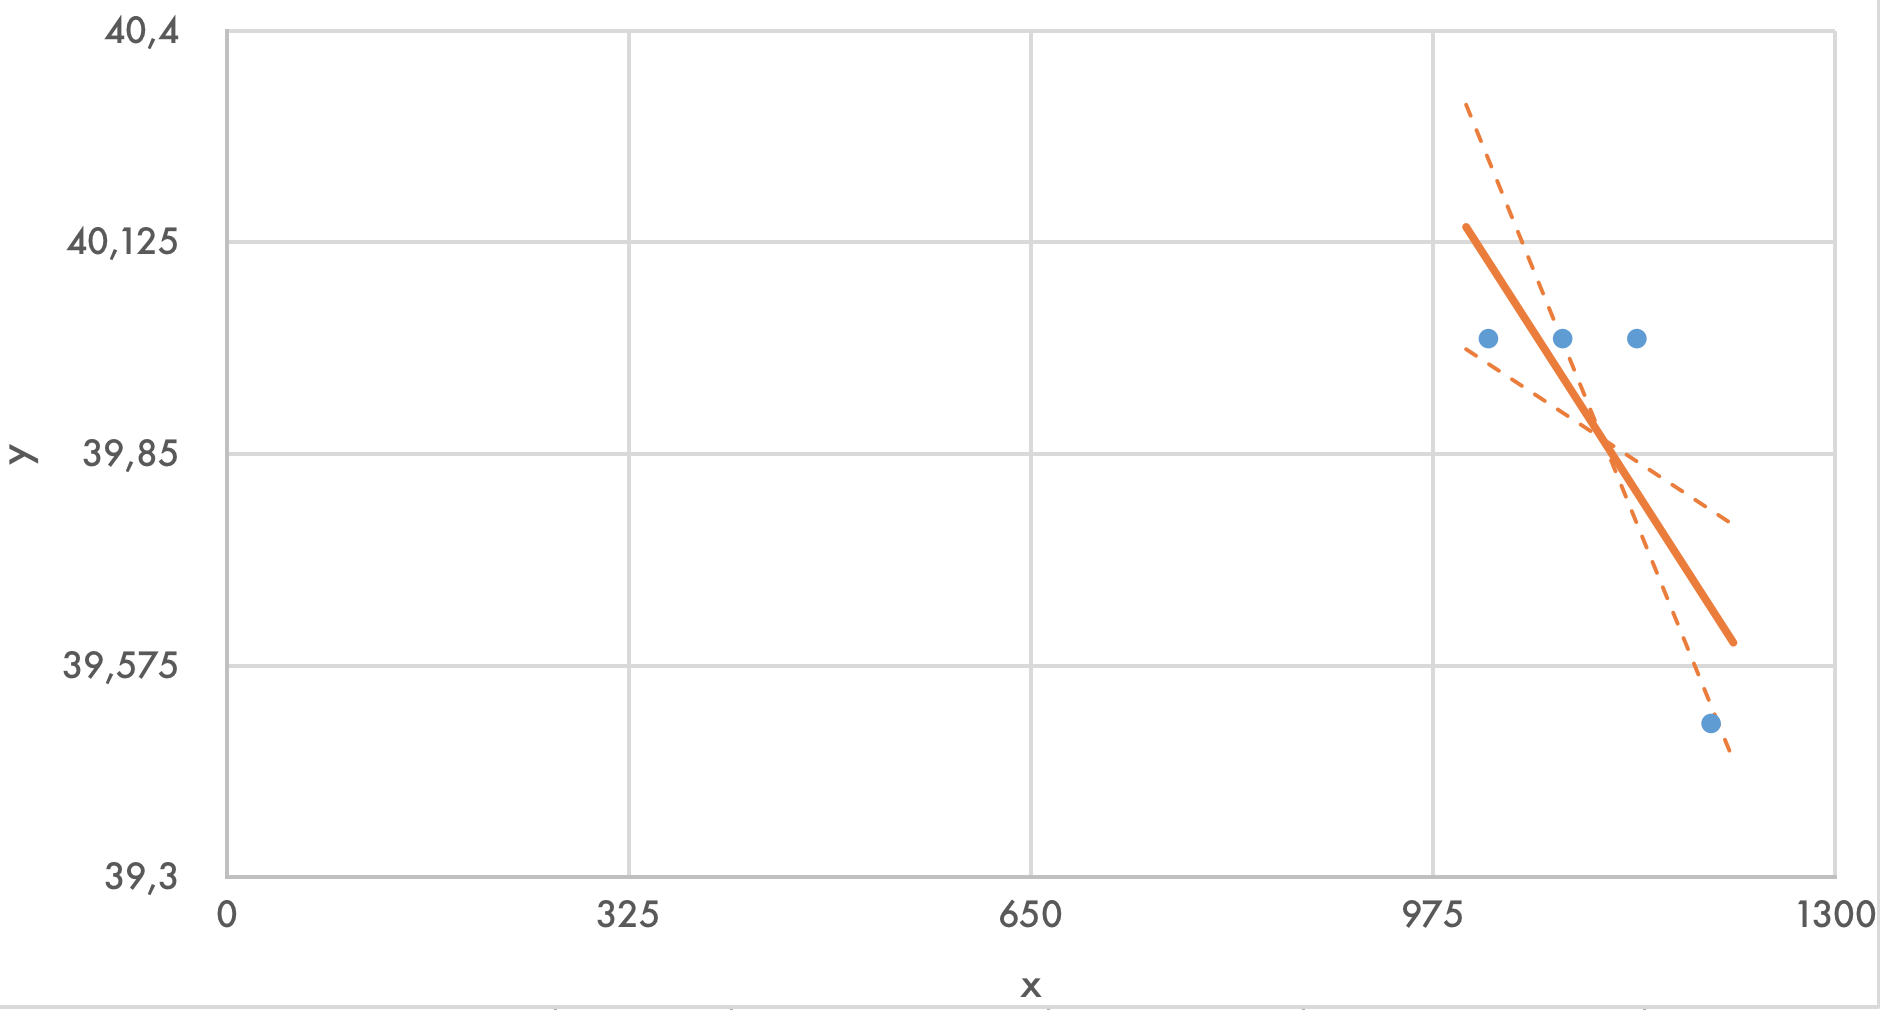
\includegraphics[width=0.7\textwidth]{extrapDia}}
   \renewcommand\thefigure{A1}
\caption{Extrapolation 2. Messreihe}
\label{Dia:1}
\end{figure}


\begin{table}[p]
	\centering
	\rowcolors{2}{gray!10}{white}
	\begin{tabular}{|r|l|}
		\multicolumn{2}{c}{\textrm{Messreihe 1}} \\
		\noalign{\global\arrayrulewidth=0.4mm}
		\hline
		\noalign{\global\arrayrulewidth=0.2mm}
		\textrm{Rotationen }$n \pm 0.3$ & \textrm{Temperatur }$T \pm 0.05\celsius$\\
		\hline
		0 & 24 \\
		10 & 24.1 \\
		20 & 24.3 \\
		30 & 24.5 \\
		40 & 24.6 \\
		50 & 24.8 \\
		\hline
	\end{tabular}
	\renewcommand\thetable{T1}
	\caption{Messreihe 1 für Teil A}
	\label{table:m1}
\end{table}

\begin{table}[p]
	\centering
	\rowcolors{2}{gray!10}{white}
	\begin{tabular}{|r|l|}
		\multicolumn{2}{c}{\textrm{Messreihe 2}} \\
		\noalign{\global\arrayrulewidth=0.4mm}
		\hline
		\noalign{\global\arrayrulewidth=0.2mm}
		\textrm{Rotationen }$n \pm 0.3$ & \textrm{Temperatur }$T \pm 0.05\celsius$\\
		\hline
		0 & 24.3 \\
		5 & 24.3 \\
		10 & 24.4 \\
		15 & 24.5 \\
		20 & 24.6 \\
		25 & 24.7 \\
		30 & 24.8 \\
		35 & 24.9 \\
		40 & 25 \\
		45 & 25.1 \\
		50 & 25.2 \\
		55 & 25.2 \\
		60 & 25.4 \\
		65 & 25.5 \\
		70 & 25.5 \\
		75 & 25.6 \\
		80 & 25.6 \\
		85 & 25.7 \\
		90 & 25.8 \\
		95 & 26 \\
		100 & 26 \\
		\hline
	\end{tabular}
	\renewcommand\thetable{T2}
	\caption{Messreihe 2 für Teil A}
	\label{table:m2}
\end{table}

\begin{table}[p]
\centering
$\begin{array}{rl}
\multicolumn{2}{c}{\textrm{\underline{Unsicherheiten:}}}\\
\textrm{Zeit: } & \pm 0.03 \textrm{s}\\
\textrm{Temperatur: } & \pm 0.02 \textrm{\celsius}\\
\textrm{Strom: } & \pm 0.03 \textrm{A}\\
\textrm{Spannung: } & \pm 0.02 \textrm{V}
\end{array}$
\rowcolors{2}{gray!10}{white}
\begin{tabular}{|c|c|c|c|}
\multicolumn{4}{l}{Wasser 116.94(3)\,g}\\
\hline
$t$ in s & $T$ in $^\circ\textrm{C}$ & $I$ in A & $U$ in V \\
\hline 
0   & 22   & 1.5 & 14.9 \\
60  & 22   & 1.5 & 14.9 \\
120 & 23   & 1.5 & 14.9 \\
180 & 24.5 & 0   & 0    \\
240 & 26.3 & 0   & 0    \\ 
300 & 26.5 & 0   & 0    \\ 
360 & 26.5 & 0   & 0	\\ 
$\vdots$ & $\vdots$ & $\vdots$ & $\vdots$ \\
2280 & 26.4 & 0 & 0 \\
\hline
\end{tabular}
\phantom{$\begin{array}{rl}
\multicolumn{2}{l}{\textrm{\underline{Unsicherheiten:}}}\\
\textrm{Zeit: } & \pm 0.03 \textrm{s}\\
\textrm{Temperatur: } & \pm 0.02 \textrm{\celsius}\\
\textrm{Strom: } & \pm 0.03 \textrm{A}\\
\textrm{Spannung: } & \pm 0.02 \textrm{V}
\end{array}$
}
\renewcommand\thetable{T4}
\caption{1. Messwerte für Teil B}
\label{tab:B1}
\end{table}

\begin{table}[p]
\centering
$\begin{array}{rl}
\multicolumn{2}{l}{\textrm{\underline{Unsicherheiten:}}}\\
\textrm{Zeit: } & \pm 0.03 \textrm{s}\\
\textrm{Temperatur: } & \pm 0.02 \textrm{\celsius}\\
\textrm{Strom: } & \pm 0.03 \textrm{A}\\
\textrm{Spannung: } & \pm 0.02 \textrm{V}
\end{array}$
\rowcolors{2}{gray!10}{white}
\begin{tabular}{|c|c|c|c|}
\multicolumn{4}{l}{Wasser 113.42(3)\,g}\\
\hline
$t$ in s & $T$ in $^\circ\textrm{C}$ & $I$ in A & $U$ in V \\
\hline 
0   & 22 & 1.5 & 14.9\\
60  & 22 & 1.5 & 14.9\\
120 & 23 & 1.5 & 14.9\\
180 & 24 & 1.5 & 14.9\\
240 & 26 & 1.5 & 14.9\\ 
300 & 27 & 1.5 & 14.9\\ 
360 & 28 & 1.5 & 14.9\\ 
420 & 29.2 & 1.5 & 14.9\\ 
480 & 30.3 & 1.5 & 14.9\\ 
540 & 31.9 & 1.5 & 14.9\\ 
600 & 33 & 1.5 & 14.9\\ 
660 & 33.7 & 1.5 & 14.9\\ 
720 & 35 & 1.5 & 14.9\\ 
780 & 35 & 1.5 & 14.9\\ 
840 & 36 & 1.5 &14.9\\
900 & 37 & 1.5 & 14.9\\
960 & 38.2 & 0 & 0\\
1020 & 39.5 & 0 & 0\\
1080 & 40 & 0 & 0\\
1140 & 40 & 0 & 0\\
1200 & 39.5 & 0 & 0\\
\hline
\end{tabular}
\phantom{$\begin{array}{rl}
\multicolumn{2}{l}{\textrm{\underline{Unsicherheiten:}}}\\
\textrm{Zeit: } & \pm 0.03 \textrm{s}\\
\textrm{Temperatur: } & \pm 0.02 \textrm{\celsius}\\
\textrm{Strom: } & \pm 0.03 \textrm{A}\\
\textrm{Spannung: } & \pm 0.02 \textrm{V}
\end{array}$
}
\renewcommand\thetable{T5}
\caption{2. Messwerte für Teil B}
\label{tab:B2}
\end{table}


\end{document}